\documentclass[aspectratio=169,11pt,hyperref={colorlinks=true}]{beamer}
\usepackage[utf8]{inputenc}
\usepackage[T1]{fontenc}
\usepackage{fontspec}
\usepackage[absolute,overlay]{textpos}
\usepackage{listingsutf8}
\usepackage{listings-golang}
\usepackage{tikz}
\usepackage{color}


\title{Developing a CD pipeline with Knative}
\date[DevOps Meetup]{March 14th 2019, Singapore, Singapore}
\author[Andrea]{
  Andrea Frittoli \\
  Developer Advocate \\
  andrea.frittoli@uk.ibm.com \\
  @blackchip76
}
\institute[DevOpsMeetupSingapore]{
  DevOps Meetup Singapore
}

\usetheme{ibmcloud}

% Code style
\setlststyle

\lstdefinelanguage{koyaml}{
  keywords={github, com, afrittoli, examples, ms, go, helloworld},
  sensitive=false,
  comment=[l]{\#},
  morestring=[b]',
  morestring=[b]"
}

% Automatic section frame
\AtBeginSection{\frame{\sectionpage}}

\begin{document}

\begin{frame}[noframenumbering]
\titlepage{}
\end{frame}

% The main points of the talk are:
% - give an introduction to Tekton Pipelines
% - get in some more details with an example
% - talk about Kaniko and source to image with tricky bits
% - reusing tasks, dev vs CI vs CD
% - point of integration with serving and eventing
% - can I use Tekton? Where? security concerns

% The slide/section order does not match the narrative yet

\section{A Bit of History}

\begin{lblackrwhiteframe}
  \frametitle{Knative}
  \large
  \begin{beamercolorbox}[wd=0.3\paperwidth]{text}
    \begin{itemize}
      \item Beginning of 2018...
      \item Knative:
      \begin{itemize}
        \item Build
        \item Eventing
        \item Serving
      \end{itemize}
    \end{itemize}
    \begin{itemize}
      \item Contributors:
      \begin{itemize}
        \item Google
        \item Pivotal
        \item IBM
        \item RedHat
        \item Cloudbees
        \item ...and others
      \end{itemize}
    \end{itemize}
  \end{beamercolorbox}%
  \begin{textblock*}{0.5\paperwidth}(0.5\paperwidth,0.2\paperheight)
    \centering
    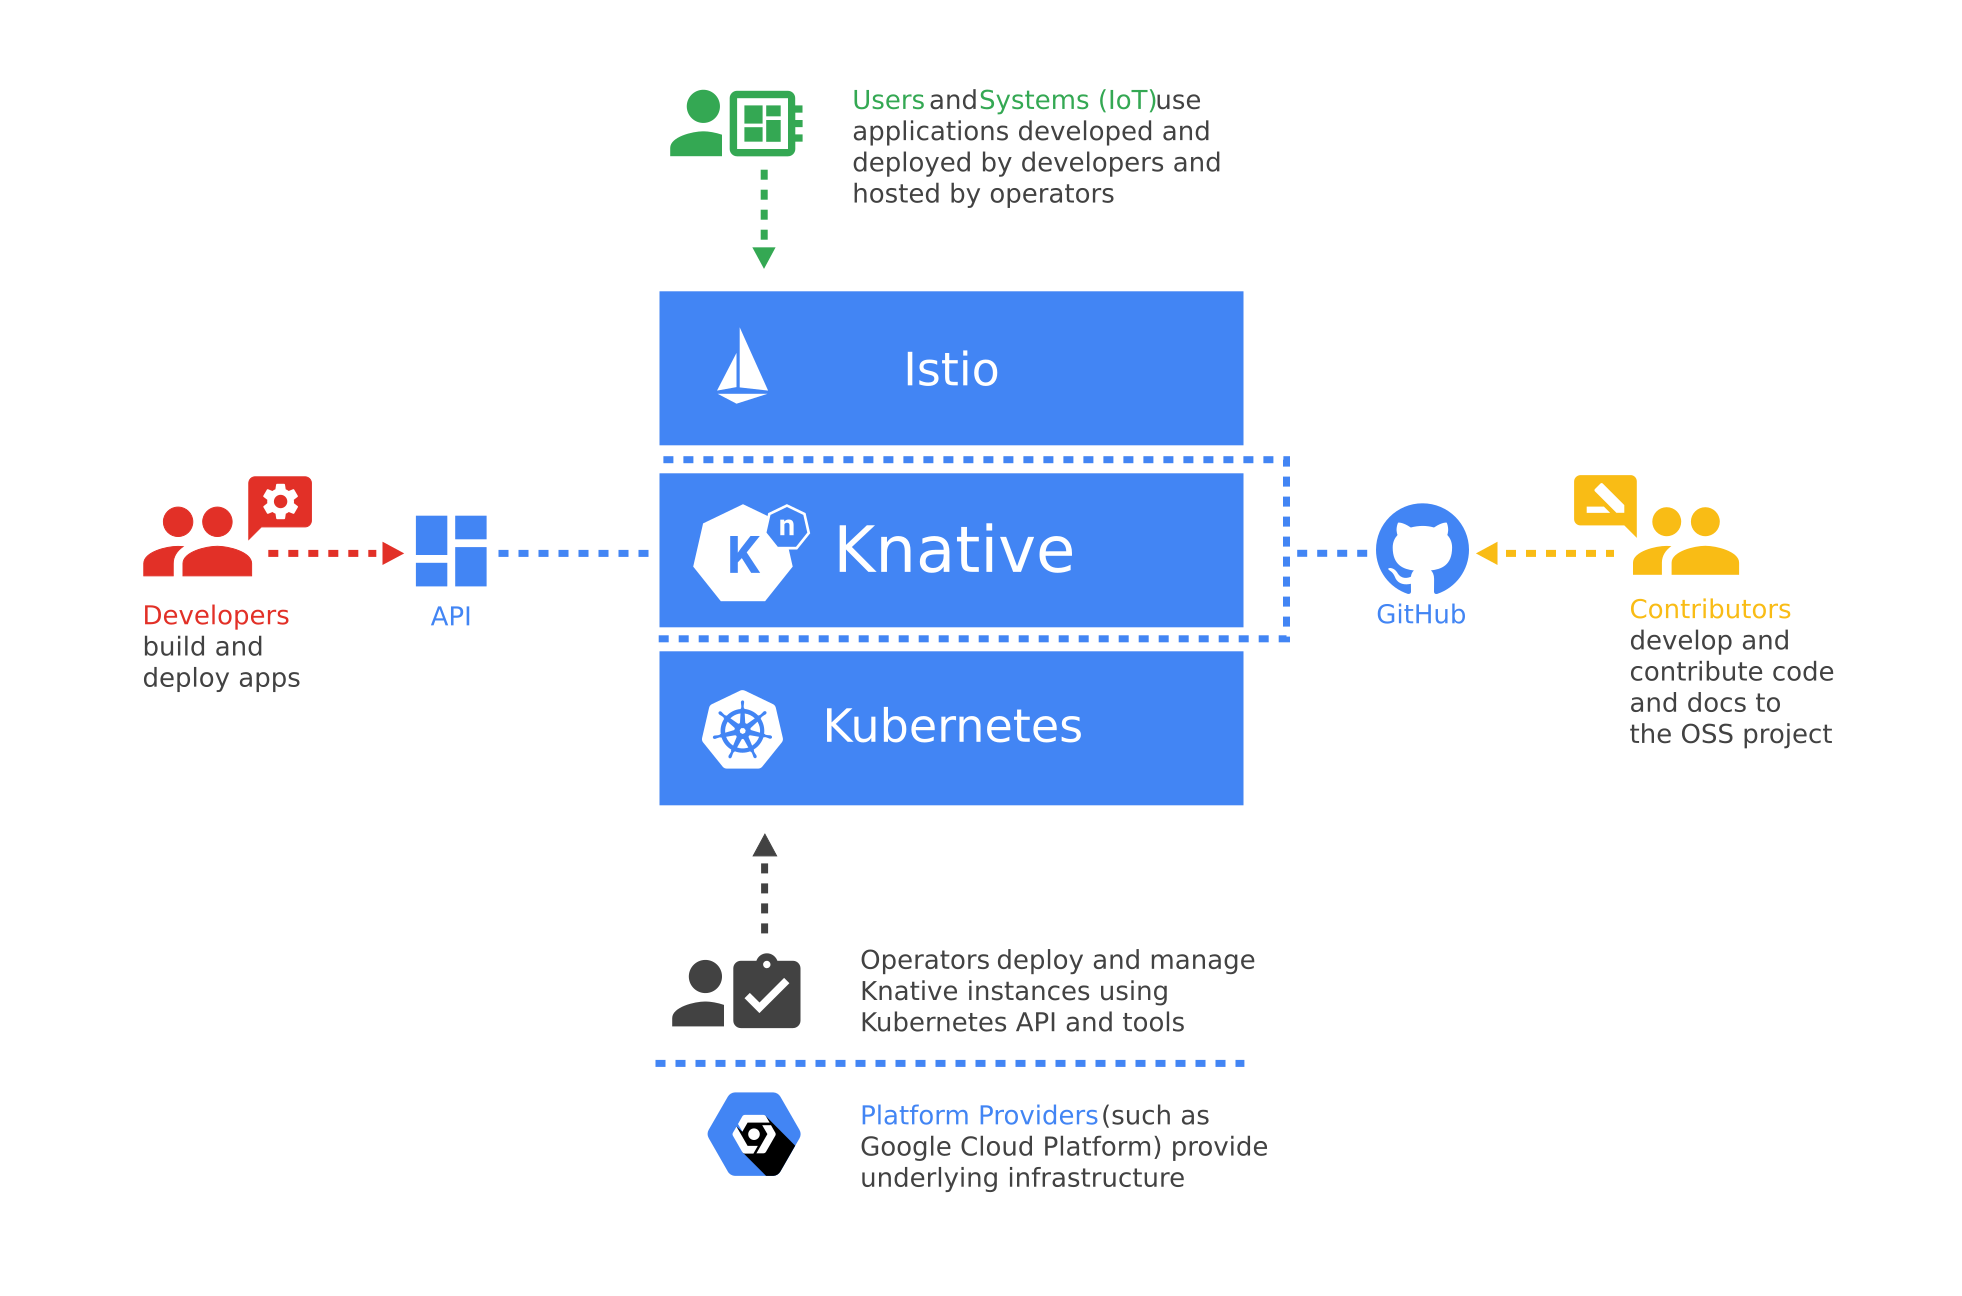
\includegraphics[width=0.45\paperwidth]{img/knative-audience.png}
  \end{textblock*}
\end{grayframe}

\begin{blackframe}
  \frametitle{\textasciitilde Sept 2018: Knative Pipelines}
  \begin{textblock*}{\paperwidth}(0cm,0.2\paperheight)
    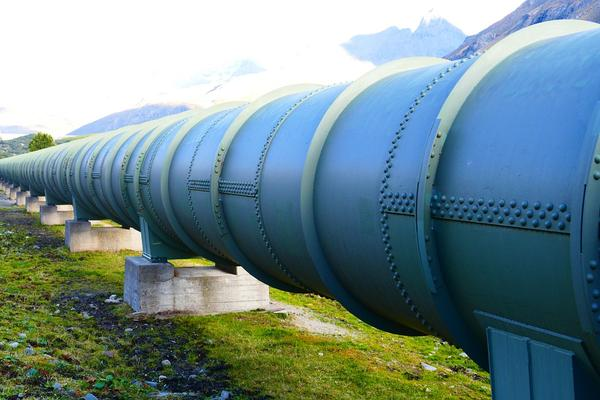
\includegraphics[width=\paperwidth]{img/pipeline_cc0.jpg}
    % https://mediad.publicbroadcasting.net/p/shared/npr/styles/placed_wide/nprshared/201804/605180710.jpg
  \end{textblock*}
  \begin{textblock*}{0.2\paperwidth}(0.83\paperwidth,0.93\paperheight)
    
\includegraphics[width=0.03\paperwidth]{img/cc.png}
    
\includegraphics[width=0.03\paperwidth]{img/zero.png}
  \end{textblock*}
\end{blackframe}

\begin{lblackrwhiteframe}
  \frametitle{Latest news!}
  \large
  \begin{beamercolorbox}[wd=0.3\paperwidth]{text}
    \begin{itemize}
      \item Focus on CI/CD
      \item Deploy ``anywhere``
      \item Compatible with Knative Build
    \end{itemize}
    \begin{itemize}
      \item {\em tektoncd/pipeline}
      \begin{itemize}
        \item New logo
        \item @CD Foundation
        \item Roadmap WIP
        \item Alpha APIs
      \end{itemize}
    \end{itemize}
  \end{beamercolorbox}%
  \begin{textblock*}{0.5\paperwidth}(0.5\paperwidth,0.25\paperheight)
    \centering
    
\includegraphics[width=0.35\paperwidth]{img/tekton-horizontal-color.png}
    
\includegraphics[width=0.20\paperwidth]{img/cdf-color.png}
  \end{textblock*}
\end{lblackrwhiteframe}

\begin{grayframe}
  \frametitle{Community}
  \begin{itemize}
    \item {\em Valid for Knative. Tekton TBD.}
    \item Steering Commitee (SC)
    \item Technical Oversight Commitee (TOC)
    \item Various Contribution profiles
    \item Design, issues: on GitHub
    \item Communication:
    \begin{itemize}
      \item Weekly video meetings, recorded, Build WG
      \item Asynch: Knative Users / Developers ML
      \item Sync: slack.knative.dev
    \end{itemize}
  \end{itemize}
\end{grayframe}

\section{Tekton Pipelines}

\begin{blackframe}
  \frametitle{Cloud Native Pipelines}
  % Cloud Native Pipelines, run on Kubernetes
  \begin{textblock*}{\paperwidth}(0.05\paperwidth,0.2\paperheight)
    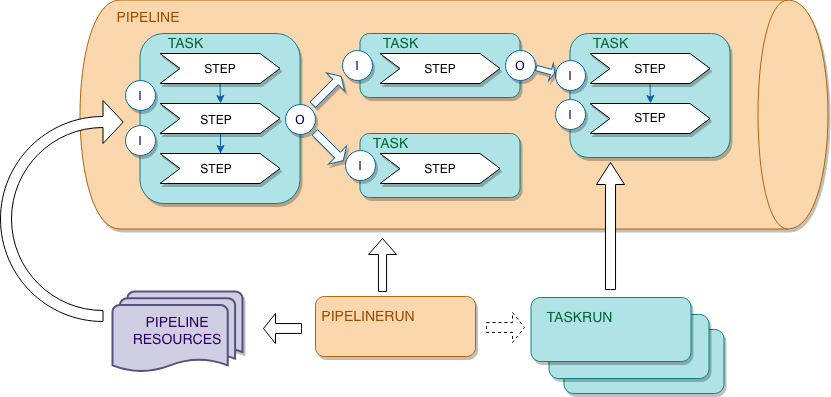
\includegraphics[width=0.85\paperwidth]{img/tekton.png}
  \end{textblock*}
  \begin{textblock*}{0.2\paperwidth}(0.9\paperwidth,0.83\paperheight)
    
\includegraphics[width=0.03\paperwidth]{img/cc.png}
    
\includegraphics[width=0.03\paperwidth]{img/zero.png}
  \end{textblock*}
\end{grayframe}

\begin{grayframe}
  \frametitle{The Health Application}
  % Talk about the architecture and git repos
  \begin{textblock*}{\paperwidth}(0cm,0cm)
    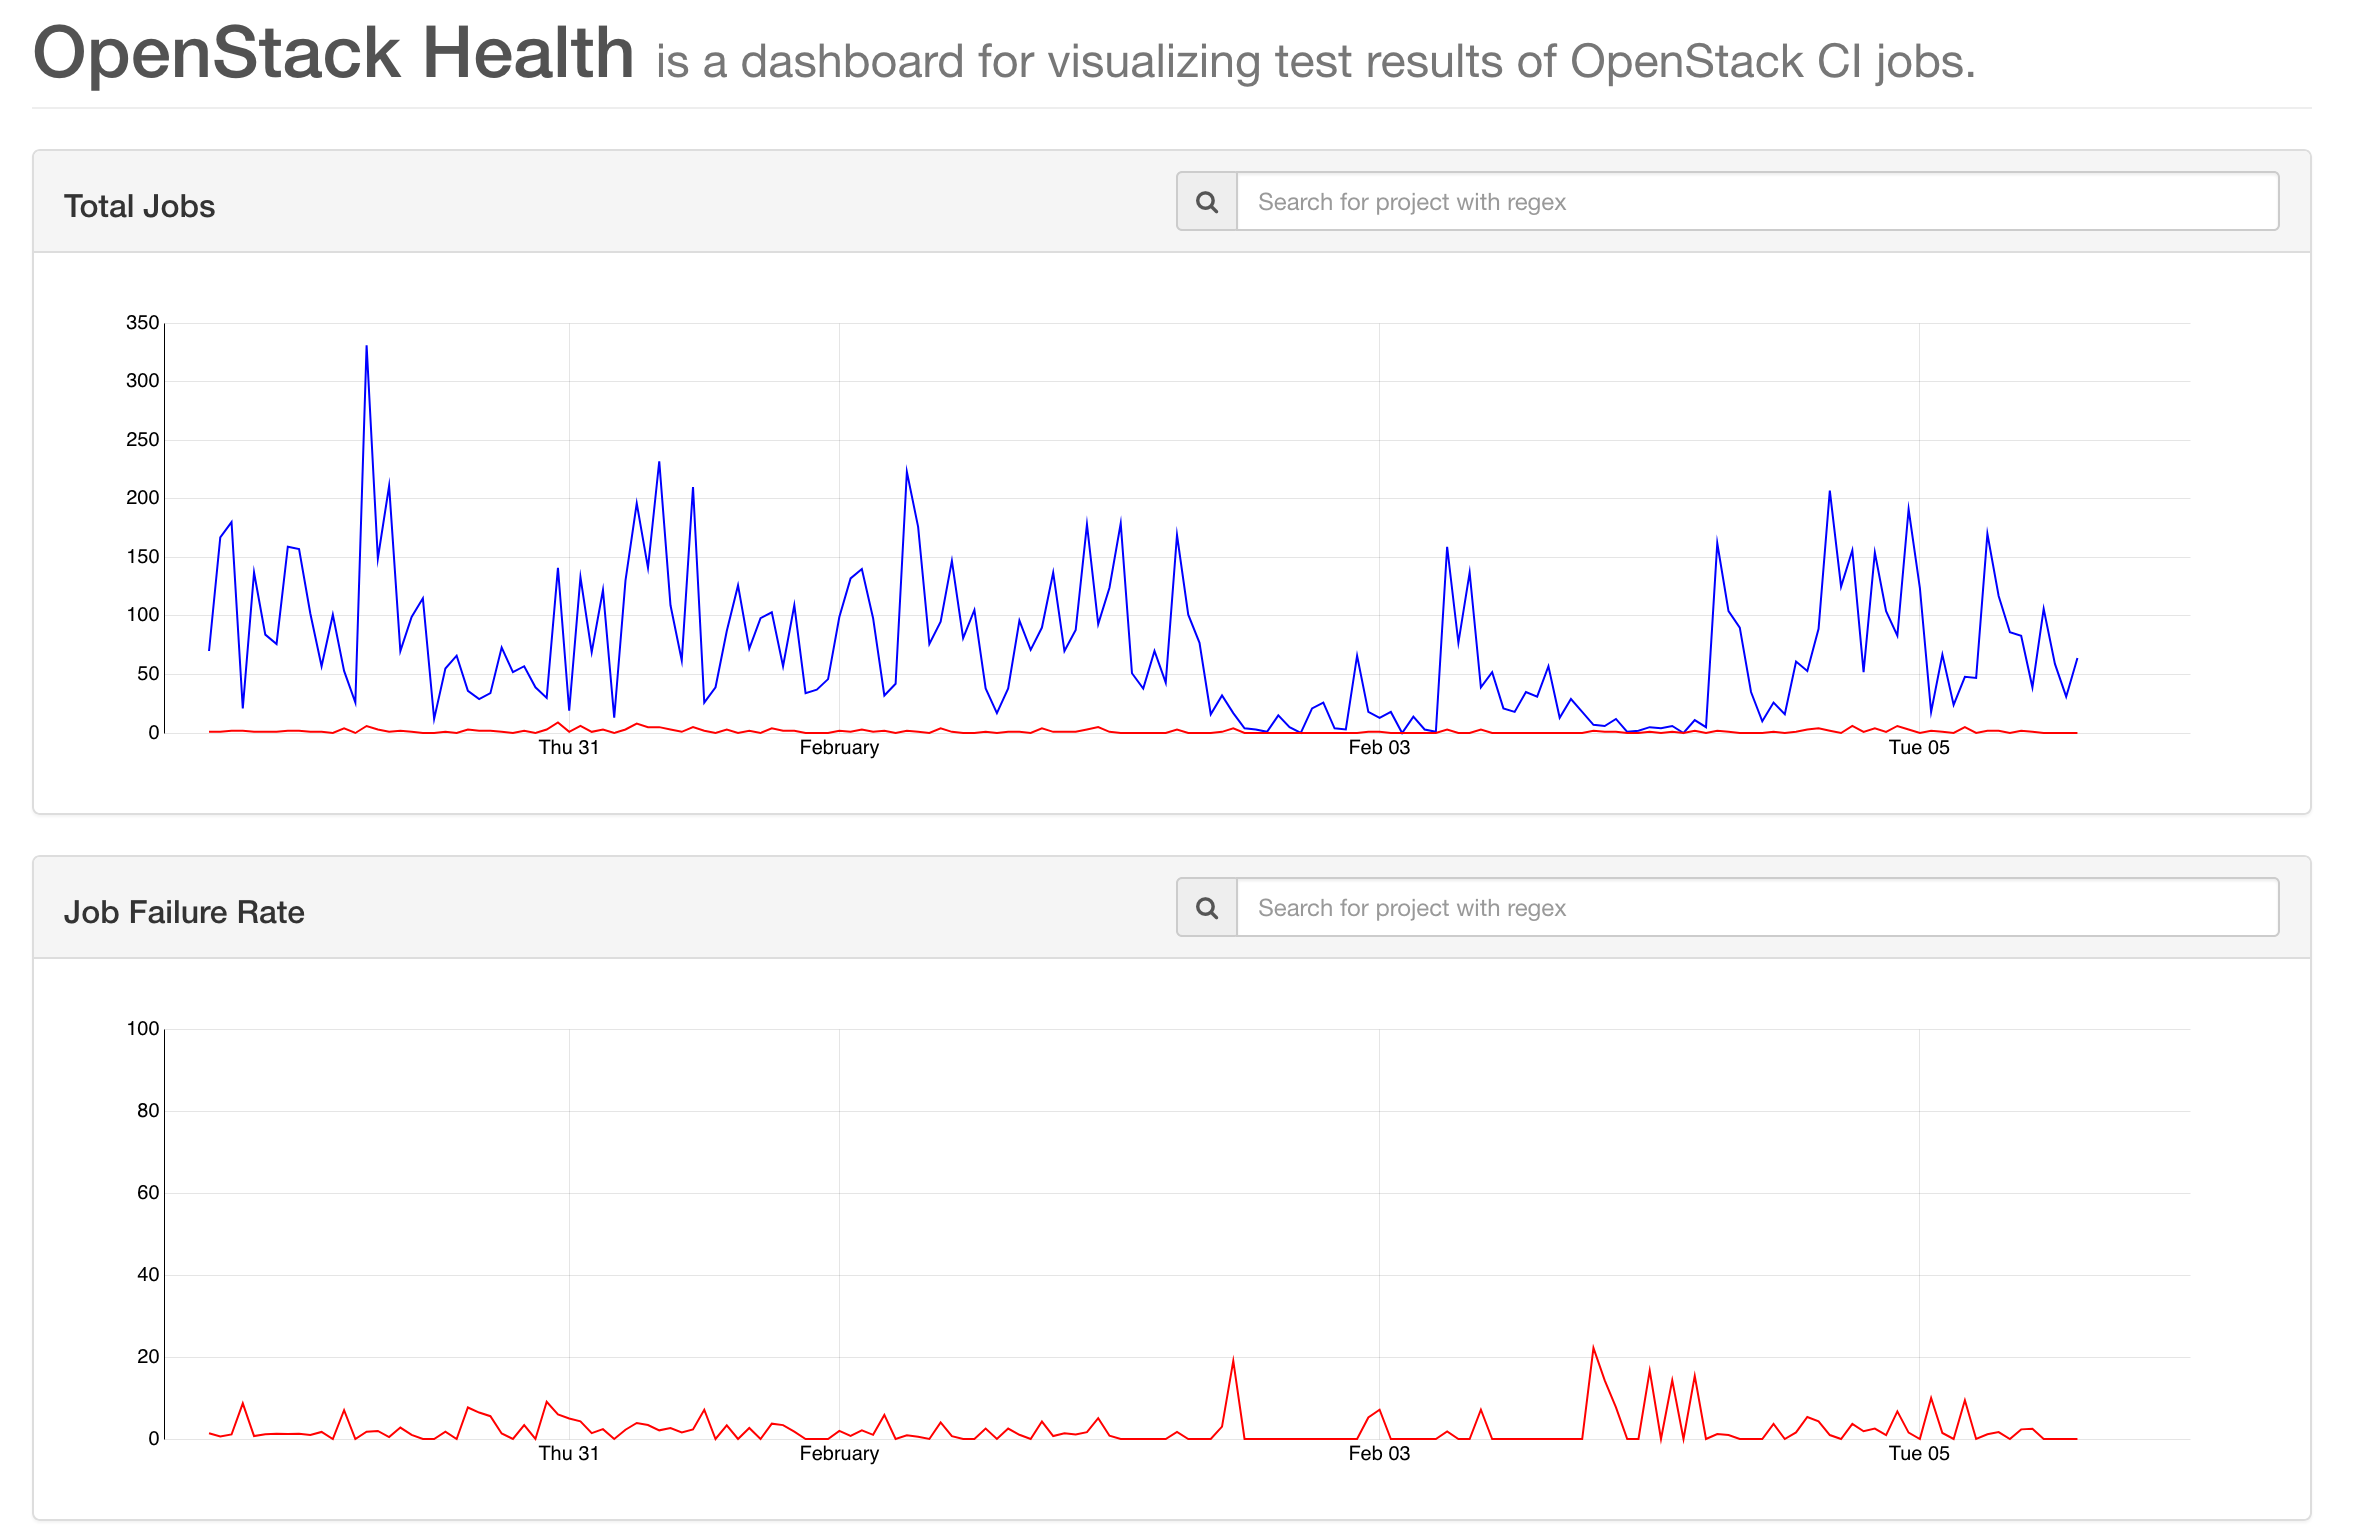
\includegraphics[width=\paperwidth, height=\paperheight]{img/openstack-health.png}
  \end{textblock*}
  \begin{textblock*}{0.2\paperwidth}(0.83\paperwidth,0.83\paperheight)
    
\includegraphics[width=0.03\paperwidth]{img/cc.png}
    
\includegraphics[width=0.03\paperwidth]{img/zero.png}
  \end{textblock*}
\end{grayframe}

\begin{2columnsframe}
  {
    \begin{itemize}
      \item Steps are sequential
      \item Tasks are a Directed Acyclic Graph
      \item Order defined by:
      \begin{itemize}
        \item {\em from}: input from another task's output
        \item {\em runAfter}: enforced task ordering
      \end{itemize}
    \end{itemize}
    % Add another pipeline example
    \begin{textblock*}{0.8\paperwidth}(0.15\paperwidth,0.50\paperheight)
      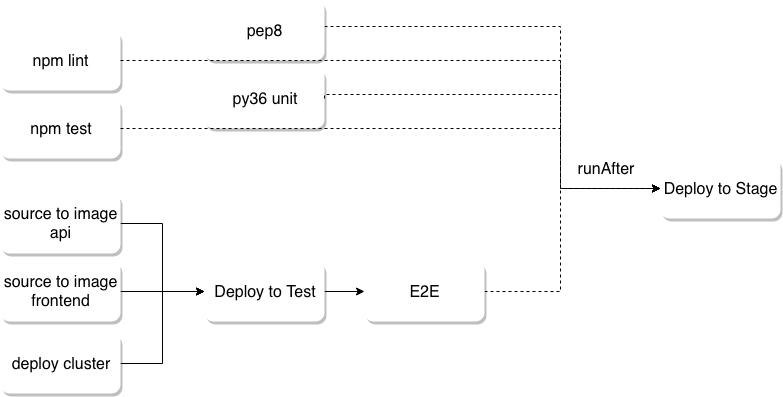
\includegraphics[width=0.45\paperwidth]{img/test-pipeline.png}
    \end{textblock*}
  }
  {
    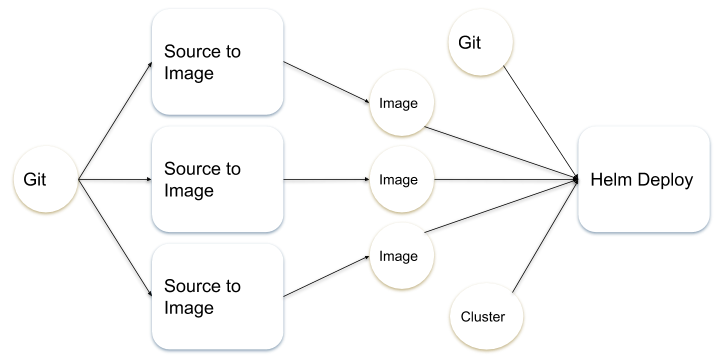
\includegraphics[width=0.4\paperwidth]{img/pipeline.png}
  }
  \frametitle{Inputs, Outputs \& DAG}
  % Graph of a simple health pipeline
\end{2columnsframe}

\section{Under the Hood}

\begin{grayframe}
  \frametitle{Custom Resources}
  CRDs: Task(Run), Pipeline(Run), PipelineResource \\
  \vspace{3ex}
  Services in the {\em tekton-pipelines} namespace:
  \begin{itemize}
    \item Webhook Service: resource validation
    \item Controller Service:
    \begin{itemize}
      \item Handles inputs and outputs
      \item Calculates the DAG
      \item Provisions pods and containers
    \end{itemize}
  \end{itemize}
  \vspace{3ex}
  Custom Resource Provisioning:
  \begin{itemize}
    \item Via YAML
    \item Via Go API
    \item Labels!
  \end{itemize}
\end{grayframe}

\begin{2columnsframe}
  {
  Steps (of a Task):
  \begin{itemize}
    \item Containers in one POD (single node)
    \item Any container image
    \item Entrypoint re-written
    \item Serial execution
    \item Resource allocation?
  \end{itemize}
  \vspace{3ex}
  TaskRun:
  \begin{itemize}
    \item Provisions a POD
    \item Deployes entrypoint tool
    \item Input/output containers
    \item User containers (steps)
  \end{itemize}
  }
  {
  Volumes:
  \begin{itemize}
    \item EmptyDir for workspace/home
    \item Tools (entrypoint)
    \item Secrets
    \item Any user ConfigMap / Volume
    \item (Optionally) Pipeline Share
  \end{itemize}
  \vspace{3ex}
  PipelineRun:
  \begin{itemize}
    \item Several PODs, different nodes
    \item Shared storage: PVC or GCS
  \end{itemize}
  }
  \frametitle{Pods, Entrypoints \& Volumes}
\end{2columnsframe}

\section{Source to Image to Deploy}

\begin{lblackrwhiteframe}
  \frametitle{IBM Cloud}
  \large
  \begin{beamercolorbox}[wd=0.4\paperwidth]{text}
    \begin{itemize}
      \item Private Registry:
      \begin{itemize}
        \item Tekon Images (push/pull)
        \item User Images (push/pull)
      \end{itemize}
      \item Service Accounts:
      \begin{itemize}
        \item {\em tekton-pipelines-controller}
        \item Pipeline/Task service account
      \end{itemize}
    \end{itemize}
    \vspace{3ex}
    \begin{itemize}
      \item Knative @ IBM Cloud
      \begin{itemize}
        \item Experimental Add-on
        \item {\em ibmcloud ks cluster-addon-enable knative}
      \end{itemize}
    \end{itemize}
  \end{beamercolorbox}%
  \begin{textblock*}{0.5\paperwidth}(0.5\paperwidth,0.3\paperheight)
    \centering
    
\includegraphics[width=0.35\paperwidth]{img/IBM-Cloud.png}
  \end{textblock*}
\end{lblackrwhiteframe}

\begin{2columnsframe}
  {
  \begin{itemize}
    \item Pipeline and Tasks in git (YAML)
    \item Parameters for env/run specific
    \item Security?
  \end{itemize}
  \vspace{3ex}
  \lstinputlisting[language=koyaml]{code/resource-git.yaml}
  }
  {
  \lstinputlisting[language=koyaml]{code/resource-cluster.yaml}
  \vspace{1ex}
  \lstinputlisting[language=koyaml]{code/resource-image.yaml}
  }
  \frametitle{CD Pipeline as code}
\end{2columnsframe}

\begin{lblackrwhiteframe}
  \frametitle{Using Kaniko}
  \large
  \begin{beamercolorbox}[wd=0.45\paperwidth]{text}
    \begin{itemize}
      \item Features:
      \begin{itemize}
        \item Build from Context and Dockerfile
        \item Unpriviledged
        \item Reproducible
        \item Remote caching of layers
        \item Base images caching (warmer)
      \end{itemize}
    \end{itemize}
    \vspace{3ex}
    \begin{itemize}
      \item Dockefile?
      \begin{itemize}
        \item Most common changes last
        \item Careful with COPY/ADD
        \item Remove what you don't need
      \end{itemize}
    \end{itemize}
  \end{beamercolorbox}%
  \begin{textblock*}{0.5\paperwidth}(0.5\paperwidth,0.25\paperheight)
    \centering
    
\includegraphics[width=0.35\paperwidth]{img/Kaniko-Logo.png}
  \end{textblock*}
\end{lblackrwhiteframe}

\begin{2columnsframe}
  {
  {\tiny Source to Image (spec only): \\}
  \lstinputlisting[language=koyaml,firstline=6,lastline=31]{code/task-source-to-image.yaml}
  }
  {
  \lstinputlisting[language=koyaml,firstline=32,lastline=55]{code/task-source-to-image.yaml}
  {\tiny Cache Warmer (spec only): \\}
  \lstinputlisting[language=koyaml,firstline=21,lastline=35]{code/task-kaniko-cache.yaml}
  }
  \frametitle{Using Kaniko}
\end{2columnsframe}
\section{Tekton and Knative}

\begin{grayframe}
  \frametitle{Pipelines and Knative Build}
  % *Run can be used as build with serving via duck typing
  % Build probably won't be developed much further
  % ...but you never know
  % Do something more complex with pipelines
  \begin{textblock*}{0.5\paperwidth}(0.20\paperwidth,0.30\paperheight)
    \centering
    
\includegraphics[width=0.6\paperwidth]{img/knative+tekton.png}
  \end{textblock*}
\end{grayframe}

\begin{grayframe}
  \frametitle{CI for OpenStack Health}
  % There's already CI, with Zuul, check it out
  % Pipeline as code... again
  % Diagram of CI pipeline for OH
  % Reusing tasks, best practices
\end{grayframe}

\begin{grayframe}
  \frametitle{CI with Tekton Pipelines}
  % It's not a CI engine...
  % ...but it works well with one
  % Dogfooding
  % What about secrets?
  % Existing integrations
  % - jenkinsX, prow
  % - gitlab? pivotal? to be checked
  % - higher level abstractions
\end{grayframe}

\section{Asynchronous Pipelines}

\begin{grayframe}
  \frametitle{Triggering and Knative Eventing}
  % Manual trigger
  % Using tasks and pipelines in Kservices
  % Native triggers: TBD
  % Async pipelines
  % GitHub events
  % -> push/pull request (CI)
  % -> comment (CI / CD)
  % -> release (CD)
\end{grayframe}

\begin{grayframe}
  \frametitle{Tekton and Development}
  % Maybe
  % Local development with minikube
  % Skaffold, ko, gulp
  % Pros and cons
  % This slide breaks the narrative here
\end{grayframe}

\section{Conclusions}

\begin{grayframe}
  \frametitle{Shall I use Tekton Pipelines?}
  % -Alpha APIs
  % +Cloud Native
  % +Relatively small footprint
  % +Momentum
  % +Reusable bits, library of Tasks
  % ...so it depends
\end{grayframe}

\begin{grayframe}
  \frametitle{Roadmap}
\end{grayframe}

\begin{grayframe}
  \frametitle{References}
  \begin{itemize}
    \item https://tekton.dev/
    \item https://github.com/tektoncd/pipeline
    \item https://cd.foundation/
    \item https://github.com/knative/docs/tree/master/community
    \item https://github.com/tektoncd/pipeline
    \item https://github.com/tektoncd/pipeline/blob/master/api\_compatibility\_policy.md
    \item https://github.com/tektoncd/pipeline/blob/master/roadmap-2019.md
    \item https://github.com/GoogleContainerTools/kaniko
    \item https://github.com/afrittoli/health-helm/tree/knative
    \item https://github.com/afrittoli/openstack-health/tree/knative-eventing
    \item https://andreafrittoli.me
    \item https://cloud.ibm.com
  \end{itemize}
\end{grayframe}

\section{Q\&A}

\end{document}
